\section{Item supplémentaire : ``Real-Time''}

Our additional item is a close attention to the computation time of deblurring. 
We develop different techniques to reduce this time and fix as objective around 1 second by picture's deblurring.  

The first point is naturally to pay attention to the implementation of our different algorithms. We try to reduce the number of nested loop, even if with color image, and image in general, loops are quite unavoidable. 

The second point is to crop the image when the whole one is unnecessary. Indeed, for the angle and length estimation of the PSF, we only need a relatively small part of a big picture and we  use the whole image for small pictures. After several tests, we conclude that a $256 \times 256 $ matrix is relevant (i.e. $\pm 1$ degree and $\pm 3$ pixels) for most of the blur and the computation time is then around maximum 0.7 second for the angle estimator and maximum 0.05 second for the length estimator, regardless the size of the initial picture. For example the figure \ref{fig:SagarShort} is computed with our crop and needs $0.684 $ [s] and $0.0463$ [s] for the angle and the length respectively whereas the figure \ref{fig:SagarLong} is computed with the whole figure and needs $11.42$ [s] and $1.128$ [s]. So the difference of time is quite big while the difference of quality is acceptable. 
\begin{figure}[h]
\centering
\begin{subfigure}{0.4\textwidth} 
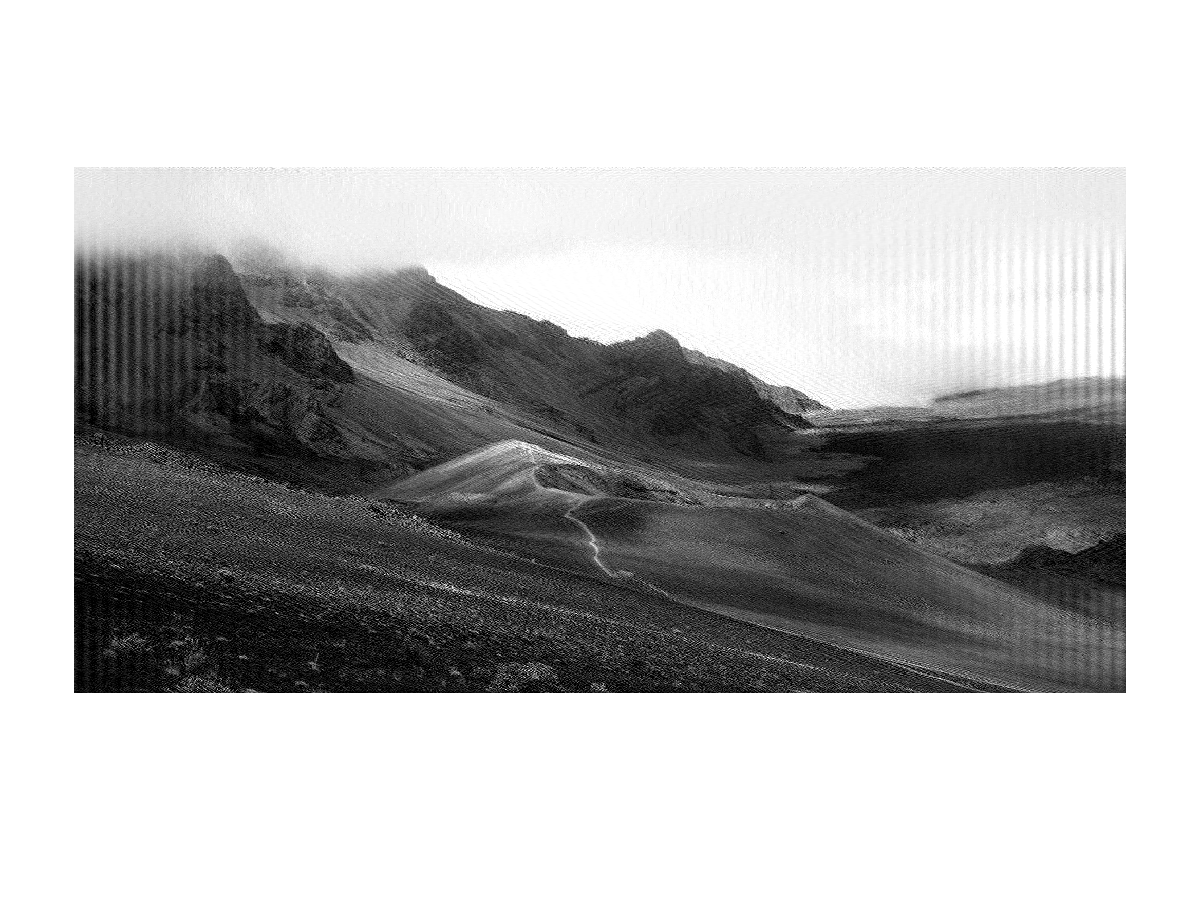
\includegraphics[width= \textwidth]{../Images/SagarShortEstimation.png}
\vspace{-30pt}
\caption{Picture deblurred using only a $256\times 256$ centered crop of the picture. }
\label{fig:SagarShort}
\end{subfigure}
~
\begin{subfigure}{0.4\textwidth}
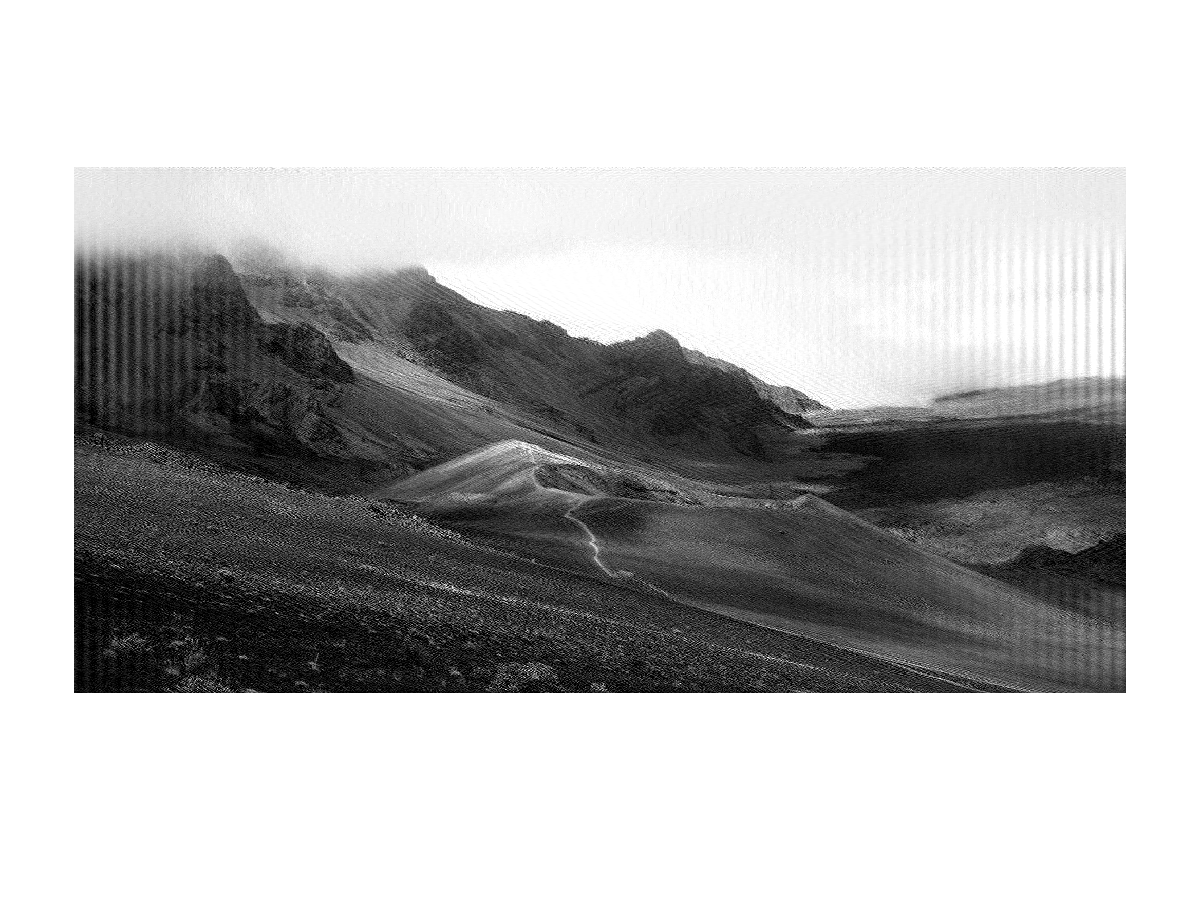
\includegraphics[{width= \textwidth}]{../Images/SagarLongEstimation.png}
\vspace{-30pt}
\caption{Picture deblurred using the whole image.}
\label{fig:SagarLong}
\end{subfigure}
\caption{Different matrix's size for the PSF estimation.}
\end{figure}

Another change is the image's resizing before the deconvolution. The goal is to reduce the number of pixels and so reduce the size of the matrix and the number of iterations needed in our loops.  However this resizing presents some challenges due to artifacts which can appear during the process. 

The main artifacts which can occur depending on the algorithm are the moiré pattern and picture's softening.  
The first one, the moiré pattern is 
\begin{figure}[h]
\centering
\begin{subfigure}{0.4\textwidth} 
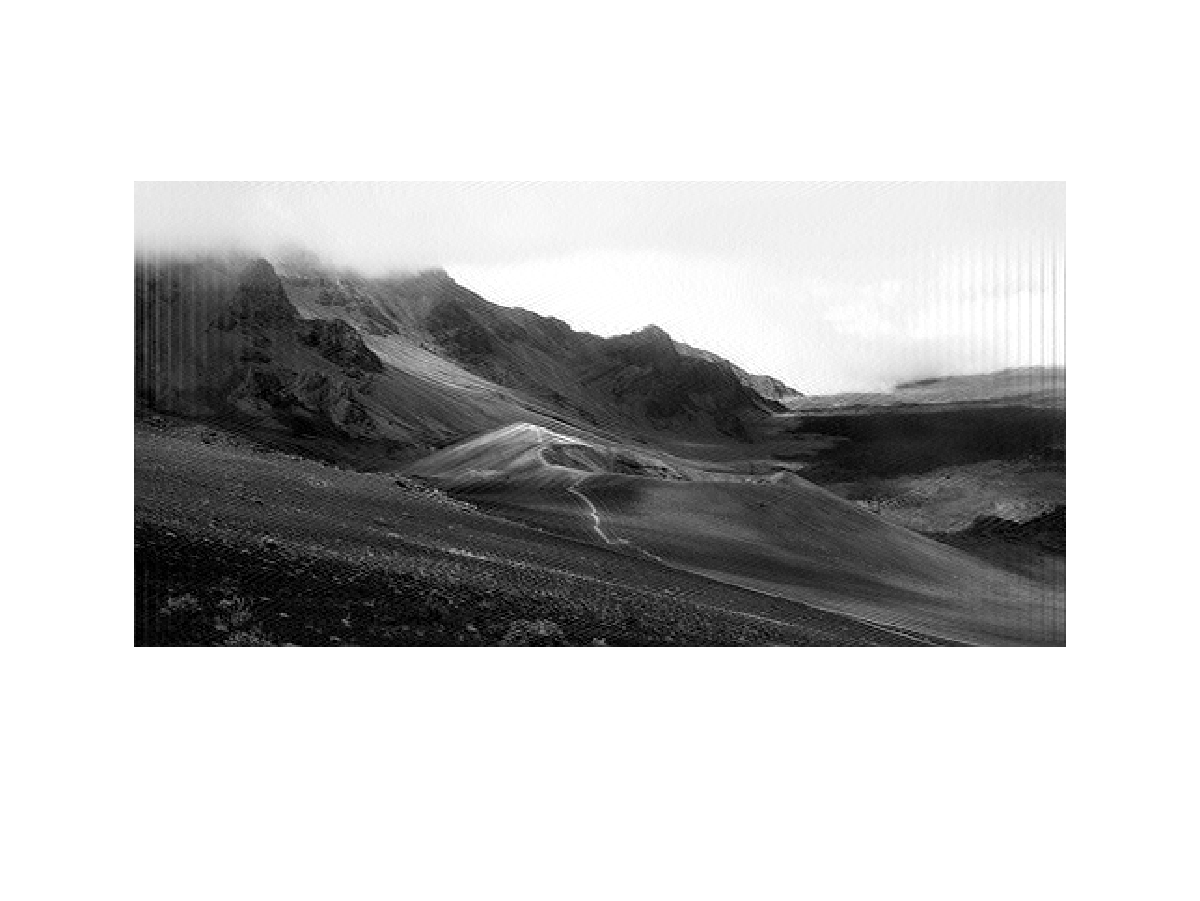
\includegraphics[width= \textwidth]{../Images/SagarLanczos3.png}
\vspace{-30pt}
\caption{Picture resized using Lanczos3 algorithm. }
\label{fig:SagarShort}
\end{subfigure}
~
\begin{subfigure}{0.4\textwidth}
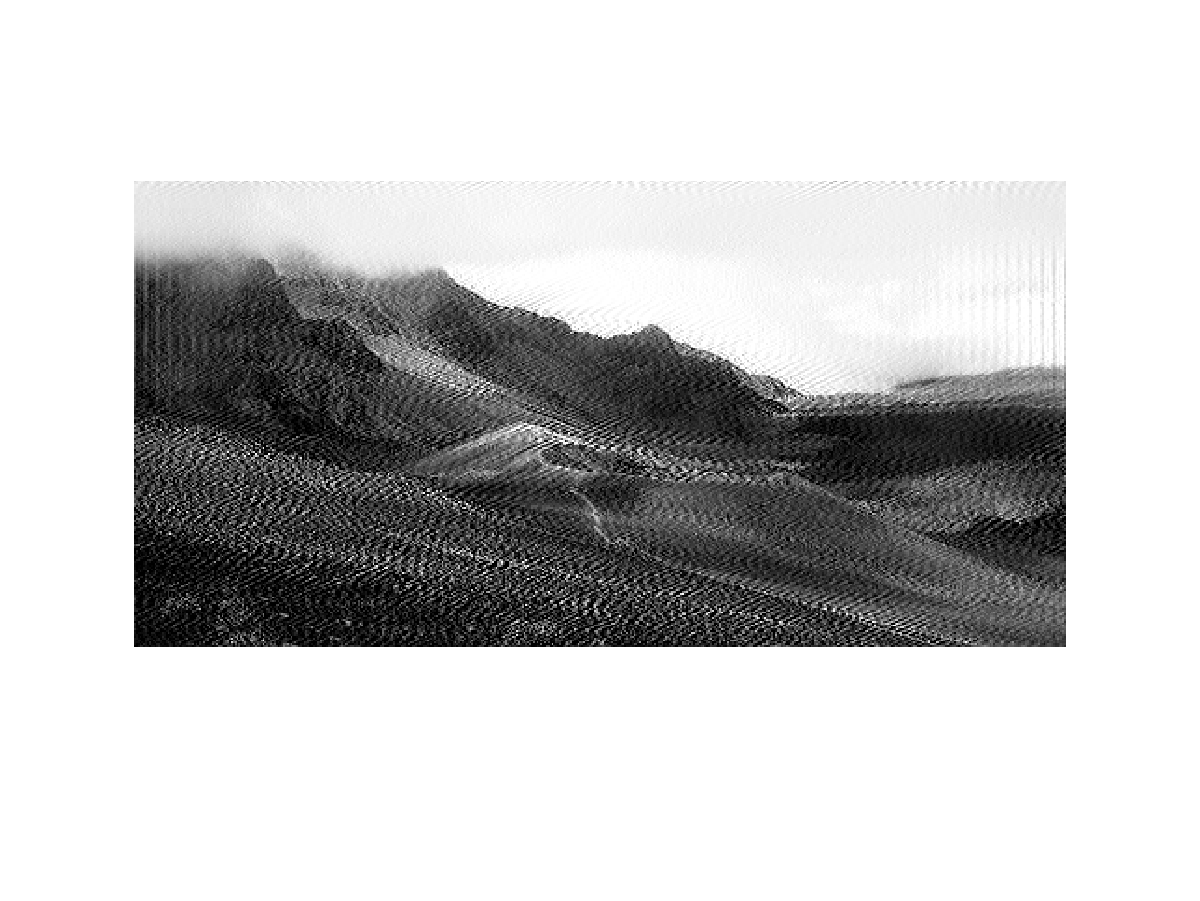
\includegraphics[{width= \textwidth}]{../Images/SagarNearest.png}
\vspace{-30pt}
\caption{Picture resized using Nearest Neighbor algorithm.}
\label{fig:SagarLong}
\end{subfigure}
\caption{Different algorithm to resize the picture.}
\end{figure}
 




%Notre critère supplémentaire est une attention particulière au temps de calcul nécessaire pour le défloutage. 
%Nous avons donc mis divers procédés en place pour réduire le temps de calcul 
%
%Comprimer l'image s'avère nécessaire dans certains cas pour ramener le temps de calcul dans des limites acceptables, et plus particulièrement pour notre item supplémentaire, le \textit{``real time''} (cf. section).



 